\ifx\pdfminorversion\undefined\else\pdfminorversion=4\fi
\documentclass[aspectratio=169,t,table]{beamer}
%\documentclass[aspectratio=169,t,handout]{beamer}

% English version FAU Logo
\usepackage[english]{babel}
% German version FAU Logo
%\usepackage[ngerman]{babel}

\usepackage[utf8]{inputenc}
\usepackage[T1]{fontenc}
\usepackage{amsmath,amssymb}
\usepackage{graphicx}
\usepackage{listings}
\usepackage{url}
\usepackage{xcolor}
\usepackage{enumitem}
\usepackage{hyperref}
\usepackage{fontawesome}
\usepackage{graphicx}
\usepackage{booktabs}
\usepackage{calc}
\usepackage{ifthen}
\usepackage{xcolor}
\usepackage{tikz}
\usepackage{tikz-cd}
\usepackage{verbatim}
\usepackage{pgfplots,pgfplotstable,pgf-pie}
\usepackage{filecontents}
\newcommand{\plots}{0.611201}
\newcommand{\plotm}{2.19882}
\pgfplotsset{height=4cm,width=8cm,compat=1.16}
\pgfmathdeclarefunction{gauss}{2}{%
  \pgfmathparse{1/(#2*sqrt(2*pi))*exp(-((x-#1)^2)/(2*#2^2))}%
}

\tikzset{
    vertex/.style = {
        circle,
        fill            = black,
        outer sep = 2pt,
        inner sep = 1pt,
    }
}

\tikzset{
    mynode/.style={
        draw,
        thick,
        anchor=south west,
        minimum width=2cm,
        minimum height=1.3cm,
        align=center,
        inner sep=0.2cm,
        outer sep=0,
        rectangle split,
        rectangle split parts=2,
        rectangle split draw splits=false},
    reverseclip/.style={
        insert path={(current page.north east) --
            (current page.south east) --
            (current page.south west) --
            (current page.north west) --
            (current page.north east)}
    }
}

\tikzset{basic/.style={
        draw,
        rectangle split,
        rectangle split parts=2,
        rectangle split part fill={blue!20,white},
        minimum width=2.5cm,
        text width=2cm,
        align=left,
        font=\itshape
    },
    Diamond/.style={ diamond,
                      draw,
                      shape aspect=2,
                      inner sep = 2pt,
                      text centered,
                      fill=blue!10!white,
                      font=\itshape
                    }}


\tikzset{level 1/.append style={sibling angle=50,level distance = 165mm}}
\tikzset{level 2/.append style={sibling angle=20,level distance = 45mm}}
\tikzset{every node/.append style={scale=1}}

\usetikzlibrary{arrows,decorations.pathmorphing,backgrounds,fit,positioning,shapes.symbols,chains,intersections,snakes,positioning,matrix,mindmap,shapes.multipart,shapes,calc,shapes.geometric}

% read in data file


\newcommand{\MaxNumberX}{3}
\newcommand{\MaxNumberY}{5}
\newcommand{\tikzmark}[1]{\tikz[remember picture] \node[coordinate] (#1) {#1};}

\pgfplotstableread{data/iris.dat}\iris
\pgfplotstablegetrowsof{\iris}
\pgfplotsset{compat=1.14}
\pgfmathsetmacro\NumRows{\pgfplotsretval-1}
\definecolor{airforceblue}{rgb}{0.36, 0.54, 0.66}

\usepgfplotslibrary{groupplots}
% Options:
%  - inst:      Institute
%                 med:      MedFak FAU theme
%                 nat:      NatFak FAU theme
%                 phil:     PhilFak FAU theme
%                 rw:       RWFak FAU theme
%                 rw-jura:  RWFak FB Jura FAU theme
%                 rw-wiso:  RWFak FB WISO FAU theme
%                 tf:       TechFak FAU theme
%  - image:     Cover image on title page
%  - plain:     Plain title page
%  - longtitle: Title page layout for long title
\usetheme[%
  image,%
  longtitle,%
  tf
]{fau}

% Enable semi-transparent animation preview
\setbeamercovered{transparent}


\lstset{%
  language=Python,
  tabsize=2,
  basicstyle=\tt,
  keywordstyle=\color{blue},
  commentstyle=\color{green!50!black},
  stringstyle=\color{red},
  numbers=left,
  numbersep=0.5em,
  xleftmargin=1em,
  numberstyle=\tt
}


% Title, authors, and date
\title[KDD]{Chapter VI: Classification}
\subtitle{Knowledge Discovery in Databases}
\author[L.~Melodia]{Luciano Melodia M.A.}
% English version
\institute[Department]{Evolutionary Data Management, Friedrich-Alexander University Erlangen-Nürnberg}
% German version
%\institute[Lehrstuhl]{Lehrstuhl, Friedrich-Alexander-Universit\"at Erlangen-N\"urnberg}
\date{Summer semester 2021}
% Set additional logo (overwrites FAU seal)
%\logo{\includegraphics[width=.15\textwidth]{themefau/art/xxx/xxx.pdf}}
\begin{document}
  % Title
  \maketitle

  {
    \setbeamertemplate{footline}{}
    \begin{frame}{Chapter VI: Classification}
        \begin{itemize}
            \item \textbf{Classification: basic concepts.}
            \item Decision-tree induction.
            \item Bayes classification methods.
            \item Rule-based classification.
            \item Model evaluation and selection.
            \item Techniques to improve classification accuracy: ensemble methods.
            \item Summary.
        \end{itemize}
    \end{frame}
  }

  {
    \setbeamertemplate{footline}{}
    \begin{frame}{Supervised vs. unsupervised learning}
        \begin{itemize}
            \item \textbf{\color{airforceblue}Supervised learning (classification).}
            \begin{itemize}
              \item Supervision:
              \begin{itemize}
                \item The \textbf{training data} (observations, measurements, etc.) are accompanied by \textbf{labels} indicating the \textbf{class} of the observations.
                \item New data is classified based on a \textbf{model} created from the training data.
              \end{itemize}
            \end{itemize}
            \item \textbf{\color{airforceblue}Unsupervised learning (clustering).}
            \begin{itemize}
              \item The class labels of training data are unknown.
              \begin{itemize}
                \item Or rather, there are no training data.
              \end{itemize}
            \end{itemize}
            \begin{itemize}
              \item Given a set of measurements, observations, etc., \\ the goal is to find classes or clusters in the data.
              \begin{itemize}
                \item See next chapter.
              \end{itemize}
            \end{itemize}
        \end{itemize}
    \end{frame}
  }

  {
    \setbeamertemplate{footline}{}
    \begin{frame}{Prediction problems: classification vs. numerical prediction}
        \begin{itemize}
            \item \textbf{Classification:}
            \begin{itemize}
              \item Predicts \textbf{\color{airforceblue}categorical class labels} (discrete, nominal).
              \item Constructs a model based on the training set and the values (class labels) in a classifying attribute and uses it in classifying new data.
            \end{itemize}
            \item \textbf{Numerical prediction:}
            \begin{itemize}
              \item Models \textbf{\color{airforceblue}continuous-valued functions}.
              \item I.e. predicts missing or unknown (future) values.
            \end{itemize}
            \item \textbf{Typical applications of classification:}
            \begin{itemize}
              \item Credit/loan approval: Will it be paid back?
              \item Medical diagnosis: Is a tumor cancerous or benign?
              \item Fraud detection: Is a transaction fraudulent or not?
              \item Web-page categorization: Which category is it?
            \end{itemize}
        \end{itemize}
    \end{frame}
  }

  {
    \setbeamertemplate{footline}{}
    \begin{frame}{Classification -- a two-step process}
        \begin{itemize}
            \item \textbf{Model construction: describing a set of predetermined classes:}
            \begin{itemize}
              \item Each tuple/sample is assumed to belong to a predefined class, as determined by the \textbf{\color{airforceblue}class-label attribute}.
              \item The set of tuples used for model construction is the \textbf{\color{airforceblue}training set}.
              \item The \textbf{\color{airforceblue}model} is represented as classification rules, decision trees, or mathematical formulae.
            \end{itemize}
            \item \textbf{Model usage, for classifying future or unknown objects:}
            \begin{itemize}
              \item Estimate \textbf{\color{airforceblue}accuracy} of the model:
              \begin{itemize}
                \item The known label of \textbf{test samples} is compared with the result from the model.
                \item \textbf{Accuracy rate} is the percentage of test-set samples that are correctly classified by the model.
                \item Test set is independent of training set (otherwise overfitting).
              \end{itemize}
              \item If the accuracy is acceptable, \textbf{\color{airforceblue}use the model} to classify data tuples whose class labels are not known.
            \end{itemize}
        \end{itemize}
    \end{frame}
  }

  {
    \setbeamertemplate{footline}{}
    \begin{frame}{Classification -- a two-step process}
      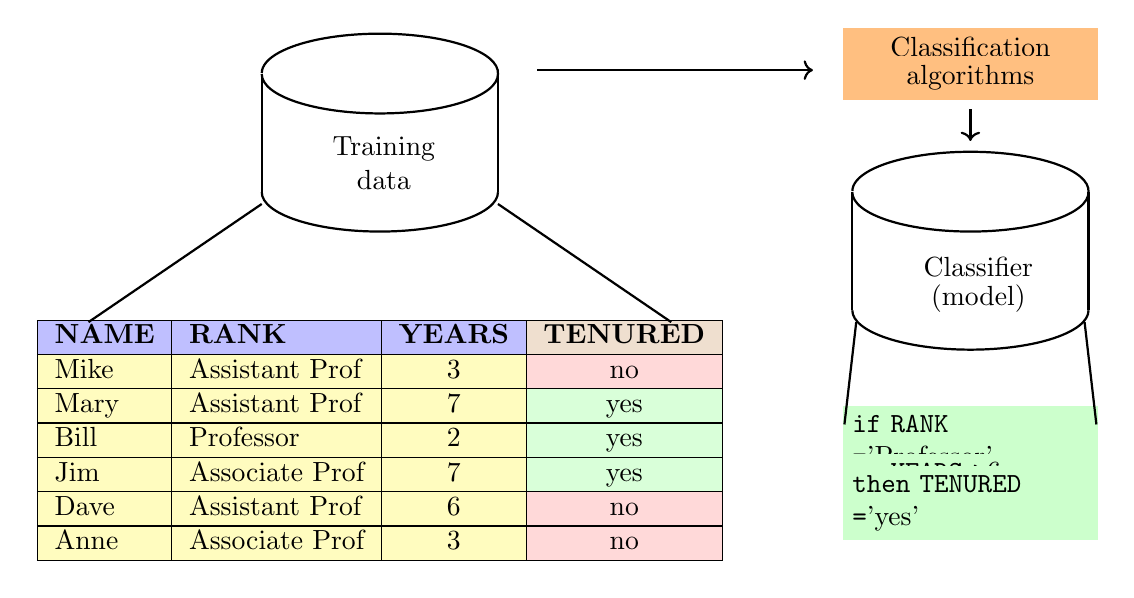
\begin{tikzpicture}
        \node at (0,0) {
        \begin{tabular}{|l|l|c|c|}
          \hline
          \cellcolor{blue!25}\textbf{\uppercase{name}} & \cellcolor{blue!25}\textbf{\uppercase{rank}} & \cellcolor{blue!25}\textbf{\uppercase{years}} & \cellcolor{brown!25}\textbf{\uppercase{tenured}} \\\hline
          \cellcolor{yellow!25}Mike & \cellcolor{yellow!25}Assistant Prof & \cellcolor{yellow!25}3 & \cellcolor{red!15}no \\\hline
          \cellcolor{yellow!25}Mary & \cellcolor{yellow!25}Assistant Prof & \cellcolor{yellow!25}7 & \cellcolor{green!15}yes \\\hline
          \cellcolor{yellow!25}Bill & \cellcolor{yellow!25}Professor & \cellcolor{yellow!25}2 & \cellcolor{green!15}yes \\\hline
          \cellcolor{yellow!25}Jim & \cellcolor{yellow!25}Associate Prof & \cellcolor{yellow!25}7 & \cellcolor{green!15}yes \\\hline
          \cellcolor{yellow!25}Dave & \cellcolor{yellow!25}Assistant Prof & \cellcolor{yellow!25}6 & \cellcolor{red!15}no \\\hline
          \cellcolor{yellow!25}Anne & \cellcolor{yellow!25}Associate Prof & \cellcolor{yellow!25}3 & \cellcolor{red!15}no \\\hline
        \end{tabular}
        };
        \node[fill=orange!50, text width = 3cm, align=center] at (7.5,5) {Classification};
        \node[fill=orange!50, text width = 3cm, align=center] at (7.5,4.6) {algorithms};


        \node[fill=green!20, text width = 3cm, align=left] at (7.5,0) {\texttt{if RANK =}'Professor'};
        \node[fill=green!20, text width = 3cm, align=left] at (7.5,-0.4) {\texttt{or YEARS >}6};
        \node[fill=green!20, text width = 3cm, align=left] at (7.5,-0.8) {\texttt{then TENURED =}'yes'};

        \node[text width = 3cm, align=center] at (0.05,3.7) {Training};
        \node[text width = 3cm, align=center] at (0.05,3.3) {data};

        \node[text width = 3cm, align=center] at (7.6,2.2) {Classifier};
        \node[text width = 3cm, align=center] at (7.6,1.8) {(model)};

        \draw [thick](-1.5,3.15) -- (-1.5,4.65);
        \draw [thick](1.5,3.15) -- (1.5,4.65);
        \draw [thick](-1.5,3.15) arc (180:360:1.5 and 0.5);
        \draw [thick](-1.5,4.65) arc (180:360:1.5 and 0.5);
        \draw [thick](1.5,4.65) arc (-1.5:180:1.5 and 0.5);
        \draw [thick, ->] (2,4.7) -- (5.5,4.7);
        \draw [thick, ->] (7.5,4.2) -- (7.5,3.8);
        \draw [thick] (6.05,1.5) -- (5.9,0.2);
        \draw [thick] (8.95,1.5) -- (9.1,0.2);

        \draw [thick](6,1.65) -- (6,3.15);
        \draw [thick](9,1.65) -- (9,3.15);
        \draw [thick](6,1.65) arc (180:360:1.5 and 0.5);
        \draw [thick](6,3.15) arc (180:360:1.5 and 0.5);
        \draw [thick](9,3.15) arc (-1.5:180:1.5 and 0.5);
        \draw [thick] (-3.7,1.5) -- (-1.5,3);
        \draw [thick] (1.5,3) -- (3.7,1.5);
      \end{tikzpicture}
    \end{frame}
  }

  {
    \setbeamertemplate{footline}{}
    \begin{frame}{Process (II): using the model in prediction}


    \end{frame}
  }

  {
    \setbeamertemplate{footline}{}
    \begin{frame}{Chapter VI: Classification}
        \begin{itemize}
            \item Classification: basic concepts.
            \item \textbf{Decision-tree induction.}
            \item Bayes classification methods.
            \item Rule-based classification.
            \item Model evaluation and selection.
            \item Techniques to improve classification accuracy: ensemble methods.
            \item Summary.
        \end{itemize}
    \end{frame}
  }

  { % Questions?
    \setbeamertemplate{footline}{}
    \begin{frame}[c]
      \begin{center}
        Thank you for your attention.\\
        {\bf Any questions about the sixt chapter?}\\[0.5cm]
        Ask them now, or again, drop me a line: \\
        \faSendO \ \texttt{luciano.melodia@fau.de}.
      \end{center}
    \end{frame}
  }
\end{document}
